\documentclass[10pt]{article}
\usepackage[a4paper,margin=2cm]{geometry}
\usepackage{booktabs,longtable,amsmath,amssymb,graphicx,caption,lscape}
\captionsetup{font=small,labelfont=bf}
\title{\bfseries Constant-Lagrangian inflow fits of the full SPARC sample:\\ overall classification of 175 rotation curves}
\author{Synthesis of the category A--E analyses, prepared for E.P.J.\ de Haas}\date{}
\begin{document}\maketitle
\section*{Summary}
This report combines the five category analyses (A--E) of the SPARC rotation curves (175 galaxies) into one physical classification. It is based only on the stored results of those analyses; nothing was refitted. Every galaxy is assigned to the simplest CL description that the respective analysis accepted, using the CL inflow model and its extensions from [1,2]. The result is:
\begin{itemize}\itemsep0pt
\item \textbf{Single-L} (100): one constant Lagrangian $(M,R)$ describes the whole curve.
\item \textbf{Double} (25): a Lagrangian reset (two-L, nested spiral) or the equivalent rising window.
\item \textbf{Single-L + descent} (24): a CL curve followed by a Keplerian descent window.
\item \textbf{Descent only} (7): the inner CL bulge is unresolved and the curve is a compact central mass plus a Keplerian descent.
\item \textbf{Multi-region} (6): two windows, or a reset plus a window.
\item \textbf{Flattening window} (2).
\item \textbf{Unresolved} (11): bulge-dominated or non-nested galaxies that the present extensions describe only with unphysical parameters.
\end{itemize}
The classes form a clear morphological sequence (Kruskal--Wallis on Hubble type for the four main classes, $p=6e-12$). Single-L and double galaxies are late types (median Sm), descent galaxies are intermediate spirals (median Sbc), descent-only and unresolved galaxies are early types (median Sb and Sab). Over the full sample the median $\chi^2_\nu$ goes from 0.86 (single-L) to 0.50 (final description) and the median RMS$_\mathrm{rel}$ in $v^2$ from 0.135 to 0.097. 19 galaxies remain at $\chi^2_\nu>2$; apart from NGC 4051 (single-L, $n=7$) all are high-precision curves, either massive bulged spirals with a sharp inner peak or well-sampled nearby disks that need more than one reset.

\section{Basis of the synthesis}
\paragraph{Models.} All descriptions use the CL inflow quantities $X=\sqrt{2GM/R}-H_zR$ and $Y(r)=\sqrt{2GM/r}-H_zr$ with $H_z=2.2\times10^{-18}\,\mathrm{s^{-1}}$, fitted to $v^2$ with $\sigma_{v^2}=2V_\mathrm{obs}\delta V_\mathrm{obs}$ (SPARC [3]).
\begin{itemize}\itemsep0pt
\item \textbf{Single-L} [2, Eqs.~17--18]: $v^2=\tfrac12X^2r^2/R^2$ for $r\le R$ and $\tfrac32X^2-Y^2$ beyond; asymptotic speed $v_L=\sqrt{3/2}X$.
\item \textbf{Two-L} [2, Eqs.~24--26]: $L_1(M_1,R_1)$ up to $R_2$, then $L_2(M_2,R_2)$.
\item \textbf{Virial window} [1, Eq.~6; 2, Eq.~19]: $+\,p[\tfrac12Y^2-\Phi_p]$ beyond $r_v$. With the continuous gauge and $H_z\to0$ this is $v^2=A+GM_N/r$, with $M_N=(p-2)M$. So $p>2$ is a Keplerian descent, $0<p<2$ a flattening and $p<0$ an additional rise.
\item \textbf{Two windows} [1, Eqs.~5--7].
\end{itemize}
\paragraph{Input analyses.} \textbf{A} (54): single-L adequate, with grades I--III. \textbf{B} (45): $+-+$ wave, two-L tested; accepted at $\Delta\mathrm{BIC}<-6$, with physical screening (nested / needs more regions / not nested). \textbf{C} (41): $-+-$ wave, virial window tested against single-L and two-L. \textbf{D} (18): other structure, five models tested. \textbf{E} (17): poor fit without detected structure (low-power runs test), extensions tested directly by BIC.
\paragraph{Assignment rules.} Each galaxy keeps the outcome of its own analysis, mapped as follows.

\begin{table}[h]\centering\small\caption{Mapping of the category outcomes to the overall classes, and counts.}\begin{tabular}{llrrrrrr}\toprule Overall class & Sub-type & A & B & C & D & E & Total\\\midrule
Single-L & adequate & 54 &  &  &  &  & 54\\
 & extra scatter ($\sigma_\mathrm{int}$) &  &  &  &  & 6 & 6\\
 & structure within errors &  &  &  & 6 &  & 6\\
 & undecided (-6$\le$dBIC$<$-2) &  & 7 &  &  &  & 7\\
 & weak $+-+$ wave &  & 15 &  &  &  & 15\\
 & weak $-+-$ wave &  &  & 12 &  &  & 12\\
\midrule
Double (two-L reset) & nested two-L &  & 13 &  &  &  & 13\\
 & rising window (p$<$0) &  &  & 1 & 1 & 5 & 7\\
 & two-L, needs more regions &  & 5 &  &  &  & 5\\
\midrule
Single-L + descent & CL + Kepler descent &  &  & 20 & 1 & 3 & 24\\
\midrule
Descent only & descent from first points &  &  &  & 1 &  & 1\\
 & descent-dominated &  &  & 6 &  &  & 6\\
\midrule
Multi-region & reset + disk window &  &  &  & 2 &  & 2\\
 & two windows &  &  &  & 2 & 2 & 4\\
\midrule
Flattening window & 0$<$p$<$2 &  &  & 2 &  &  & 2\\
\midrule
Unresolved (bulge / non-nested) & extreme window parameters &  &  &  & 5 & 1 & 6\\
 & two-L non-nested &  & 5 &  &  &  & 5\\
\midrule
Total & & 54 & 45 & 41 & 18 & 17 & 175\\\bottomrule\end{tabular}\end{table}
\noindent Descent galaxies from C are labelled \emph{descent only} when no data point lies inside the fitted CL bulge radius and $p\ge30$ (inner Lagrangian mass negligible against $M_N$), or when at most two points precede $r_v$. NGC 7814 (D) is assigned to this class because its descent starts at the first data points.

\begin{figure}[h]\centering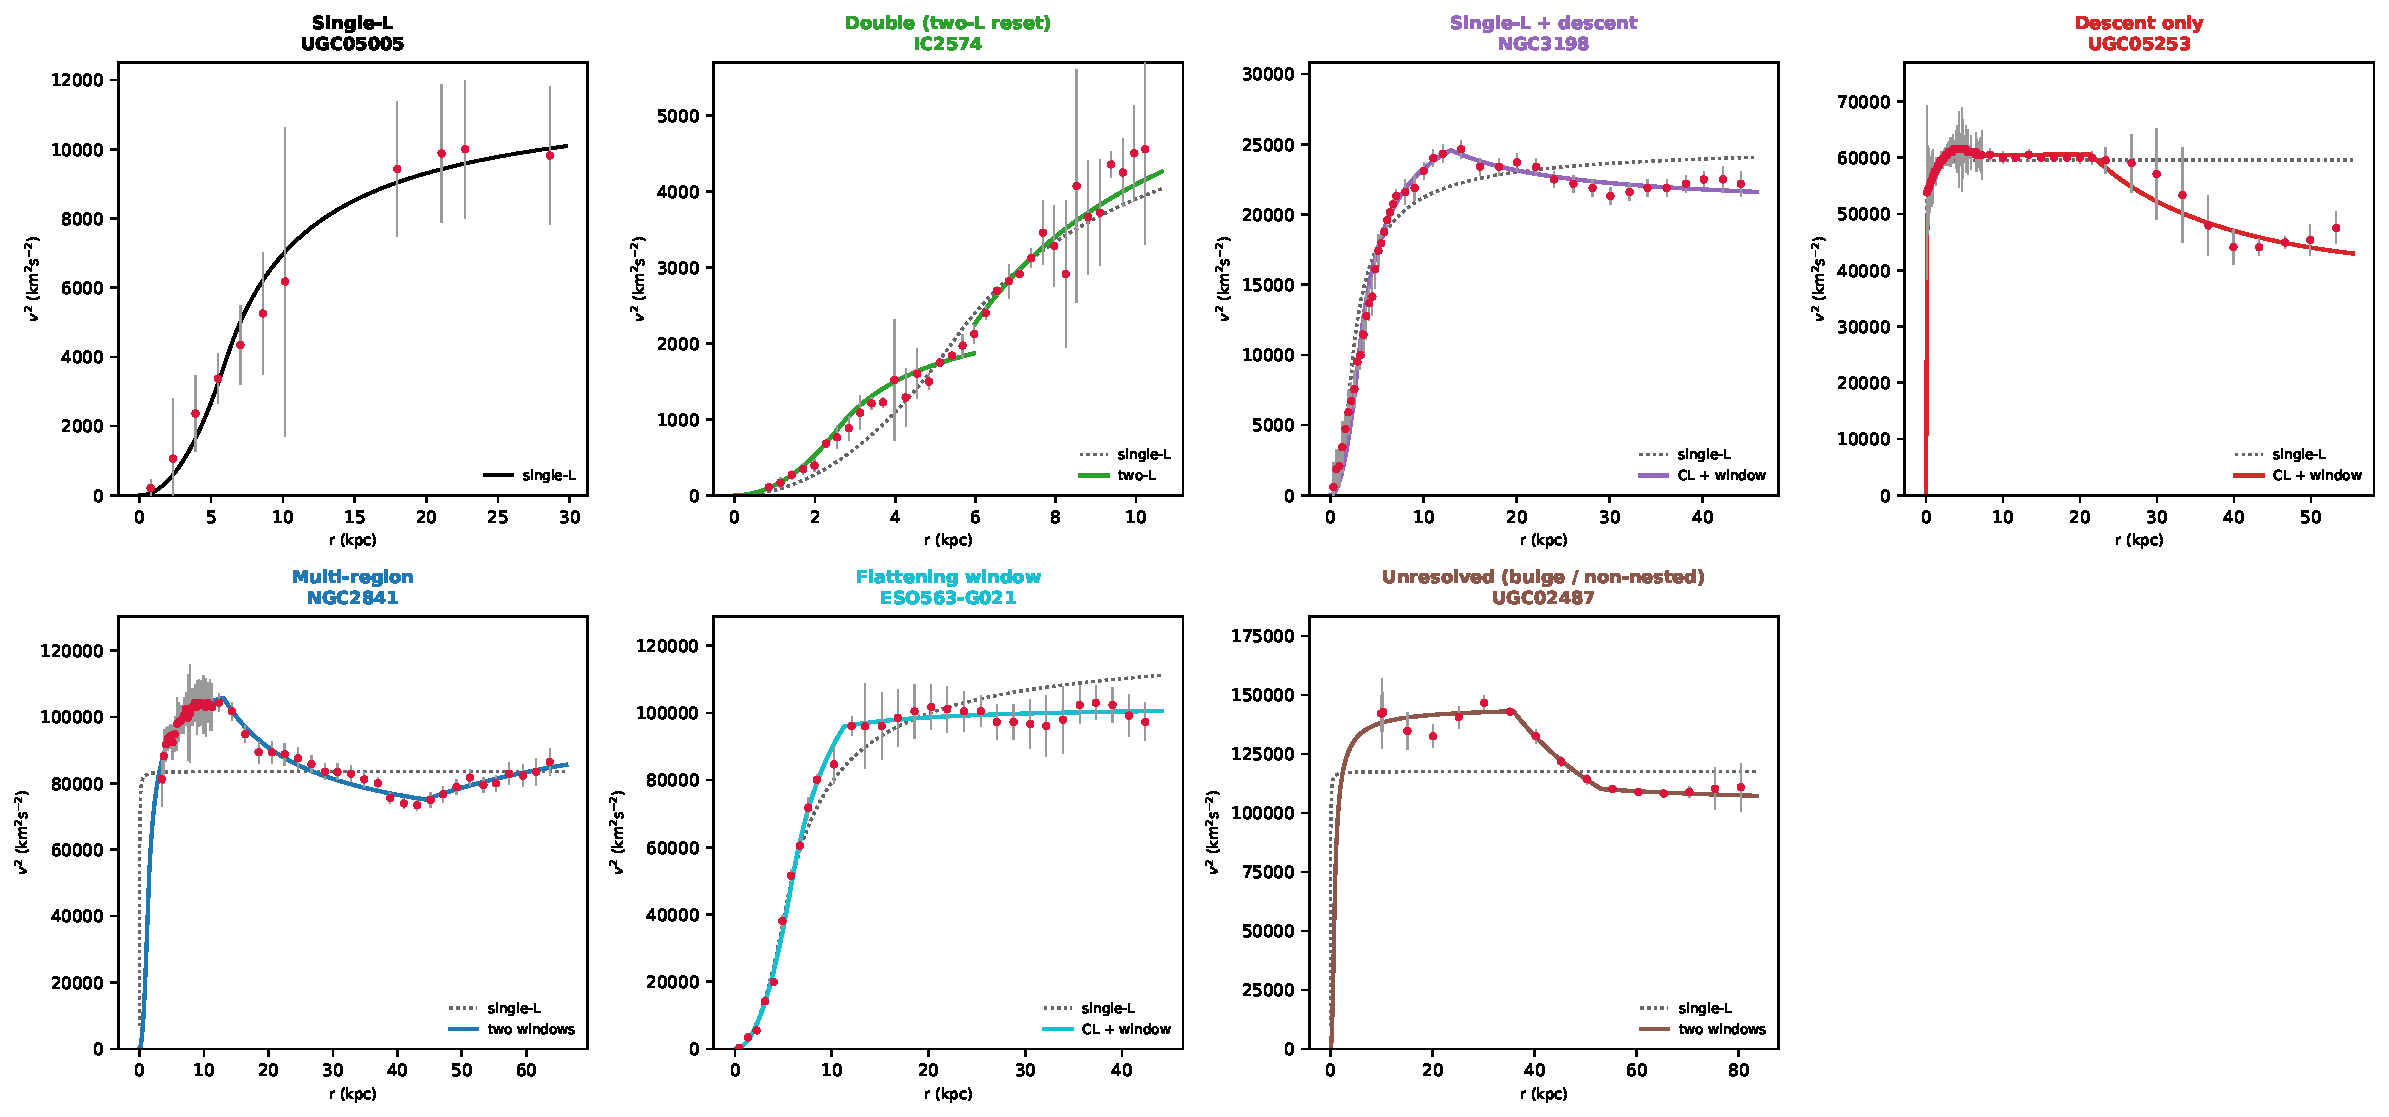
\includegraphics[width=\textwidth]{overall_fig_gallery.pdf}\caption{One representative per class, drawn from the stored best fits (dotted: single-L; solid: final description).}\end{figure}
\section{The classes}
\subsection{Single-L (100)}
$n$ median 10; $\chi^2_\nu$ 0.28$\to$0.28; RMS$_\mathrm{rel}$ 0.109$\to$0.109; Q=1: 47/100; final $\chi^2_\nu>2$: 1; $n\le13$ (tentative): 69; asymptotic speed/$V_\mathrm{flat}$ = 1.08 ($r$=0.99, 58 galaxies).

One constant Lagrangian describes the full rotation curve. The class consists of the 54 category-A galaxies plus 46 galaxies from B--E whose residual structure, although detectable in sign, does not justify extra parameters ($\Delta\mathrm{BIC}\ge-6$). These comprise 7 B galaxies with positive but not strong evidence for a reset (NGC 3109, NGC 3972, NGC 4010, UGC 6446, UGC 7125, UGC 7323, UGC 7399), weak waves in B and C, structure within the errors in D, and E galaxies whose excess $\chi^2$ corresponds to an intrinsic scatter of a few km\,s$^{-1}$. The class is dominated by late types and dwarfs (median Sm; 55 Sm/Im/BCD). The curves are short: 69 of 100 have $n\le13$, so ``single-L adequate'' often means that the data cannot demand more. The best-determined quantity is $v_L$, which tracks $V_\mathrm{flat}$ closely. $M$ and $R$ are strongly correlated (category-A median $\rho_{MR}=0.97$), and only 17 category-A galaxies have both determined to better than 30\% (grade I).

\subsection{Double: Lagrangian reset (25)}
$n$ median 21; $\chi^2_\nu$ 3.26$\to$0.90; RMS$_\mathrm{rel}$ 0.249$\to$0.127; Q=1: 16/25; final $\chi^2_\nu>2$: 6; $n\le13$ (tentative): 8; asymptotic speed/$V_\mathrm{flat}$ = 1.14 ($r$=0.95, 16 galaxies).

The rotation curve switches from an inner Lagrangian (bulge/bar zone, $L_1$) to an outer one (disk, $L_2$) at $R_2$, the nested-spiral configuration. The class contains the 13 clean nested two-L galaxies of B, the 5 B galaxies improved by two-L but needing further regions (DDO154, NGC1003, NGC2403, NGC5585, UGC03580), and 7 galaxies from C, D and E where a rising window ($p<0$) is preferred; in most of these the two-L fit is statistically equivalent. It is the late-type class (median Sm, 20 of 25 Sd--Im; photometric bulge in 2). Typical scales: $R_1/R_2\approx0.3$, $M_2/M_1\approx8$, $v_{L2}/v_{L1}\approx1.6$, $R_2$ at 1--4 disk scale lengths. Caveat: $R_2$ is a discontinuity location and is localised only to the gap between data points; the size of the $v^2$ jump is not constrained by the data.

\subsection{Single-L + descent (24)}
$n$ median 29; $\chi^2_\nu$ 4.28$\to$0.89; RMS$_\mathrm{rel}$ 0.149$\to$0.075; Q=1: 18/24; final $\chi^2_\nu>2$: 5; $n\le13$ (tentative): 6; asymptotic speed/$V_\mathrm{flat}$ = 0.94 ($r$=0.96, 20 galaxies).

A CL rise and peak followed, beyond $r_v$, by a Keplerian descent $v^2=A+GM_N/r$ onto a floor $A$. These are intermediate spirals (median Sbc; photometric bulge in 10 of 24). The descent starts at $r_v\approx$ 3--4 disk scale lengths, just beyond the peak. The floor and window radius are well determined (category C: 6\% and 9\%), the descent mass less so (23\%), and the descent mass is of order of the baryonic mass. The virial strength $p$ ranges widely (category C: $p\approx3.8$--60, 16--84\%); the pure Kepler case $p=3$ is one end of this range, not the rule. Residual structure remains in 12 galaxies, located at the inner peak of high-precision curves.

\subsection{Descent only (7)}
$n$ median 19; $\chi^2_\nu$ 5.54$\to$1.06; RMS$_\mathrm{rel}$ 0.114$\to$0.053; Q=1: 5/7; final $\chi^2_\nu>2$: 2; $n\le13$ (tentative): 0; asymptotic speed/$V_\mathrm{flat}$ = 0.80 ($r$=0.98, 6 galaxies).

NGC0891, NGC5033, NGC5371, NGC6674, UGC02916, UGC05253, NGC7814. All are Sab--Sc spirals (Sb, Sc, Sbc, Sb, Sab, Sab, Sab), with a photometric bulge in 6 of 7. The inner CL Lagrangian is not resolved: its radius lies inside the first data point, or the descent begins at the first points. The curve is described by a compact central mass with a Keplerian descent onto a floor. The quantities $r_v$, $A$ and $M_N$ are well defined; $M$, $R$ and $p$ are not. The floor lies well below $V_\mathrm{flat}$ (median ratio 0.80) because these curves are still descending at the last point. This class is the direct successor of the earlier descent-only fits; with the window formulation the parameters are positive and remain defined for $H_z\neq0$.

\subsection{Multi-region (6)}
$n$ median 23; $\chi^2_\nu$ 4.94$\to$1.14; RMS$_\mathrm{rel}$ 0.133$\to$0.052; Q=1: 4/6; final $\chi^2_\nu>2$: 1; $n\le13$ (tentative): 1.

NGC1090, NGC2841, NGC6015, UGC00128, NGC6195, UGC05764. These need two windows or a reset plus a window. NGC 2841 (descent at 13\,kpc, renewed rise at 44\,kpc) and NGC 6015 (reset at 2.3\,kpc, flattening at 3.5\,kpc) are clean examples of the multi-region configurations of [1]. The others are improved but weakly constrained.

\subsection{Flattening window (2)}
$n$ median 31; $\chi^2_\nu$ 2.34$\to$0.76; RMS$_\mathrm{rel}$ 0.099$\to$0.070; Q=1: 2/2; final $\chi^2_\nu>2$: 0; $n\le13$ (tentative): 0.

ESO563-G021 and IC 4202 (Sbc, edge-on): beyond $r_v\approx10$\,kpc the curve rises more slowly than single-L ($0<p<2$), with no descent.

\subsection{Unresolved (11)}
$n$ median 28; $\chi^2_\nu$ 3.06$\to$0.80; RMS$_\mathrm{rel}$ 0.125$\to$0.058; Q=1: 7/11; final $\chi^2_\nu>2$: 4; $n\le13$ (tentative): 2.

NGC3726, NGC4013, UGC02885, UGC06614, UGC06787, NGC0289, UGC02487, UGC03546, UGC06786, UGC09133, NGC2955. All are early or intermediate types (S0--Sc, median Sab), with a photometric bulge in 9 of 11. Statistically the extensions improve them strongly, but only with non-nested resets (a $v^2$ drop at $R_2$, or $M_2<M_1$) or extreme window strengths with the CL bulge radius at its lower bound. Their residuals trace a sharp inner peak that the parabolic CL bulge ($v^2\propto r^2$ inside $R$) cannot follow. This class marks the present limit of the model, not a separate dynamical regime.
\section{Morphological sequence}
\begin{figure}[h]\centering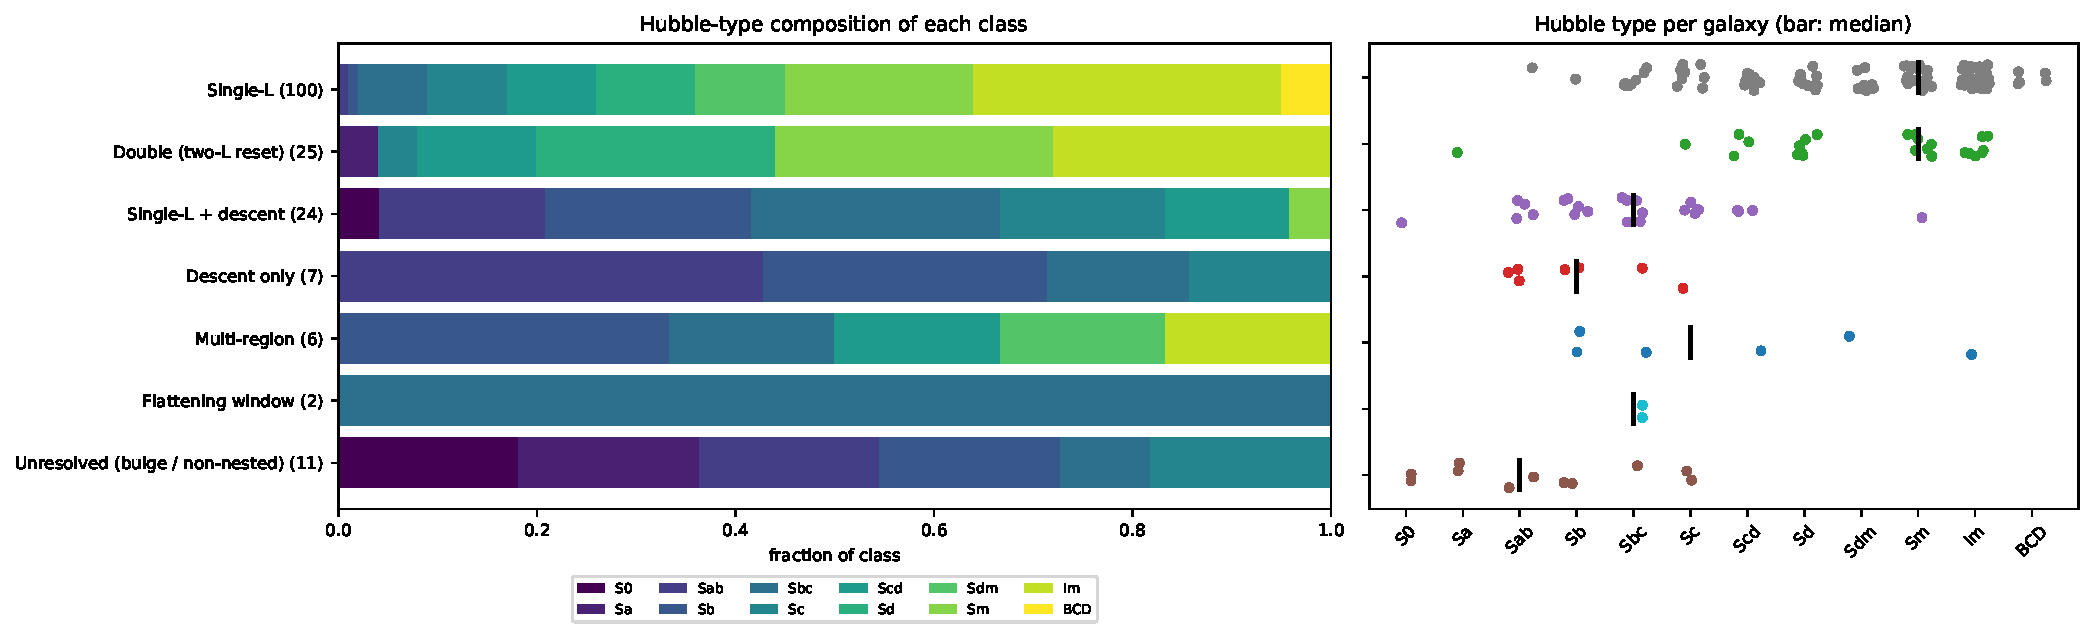
\includegraphics[width=\textwidth]{overall_fig_morphology.pdf}\caption{Hubble-type composition of the classes (left) and Hubble type per galaxy (right; bar = median).}\end{figure}
The classes are ordered in morphology (Fig.~2). Single-L and double galaxies are late types and dwarfs (medians Sm and Sm). Single-L + descent galaxies are intermediate spirals (median Sbc). Descent-only and unresolved galaxies are the earliest types (medians Sb and Sab). The difference between the four main classes is highly significant (Kruskal--Wallis $H=55.3$, $p=6e-12$). The fraction of galaxies with a photometric bulge rises along the same sequence: 2% (single-L), 8% (double), 42% (single + descent), 86% (descent only), 82% (unresolved). In CL terms: bulgeless disks either keep one Lagrangian or reset to a second one, bulged spirals develop a Keplerian descent beyond the peak, and bulge-dominated systems are descent-dominated or exceed the present bulge description.
\section{Global fit quality}
\begin{figure}[h]\centering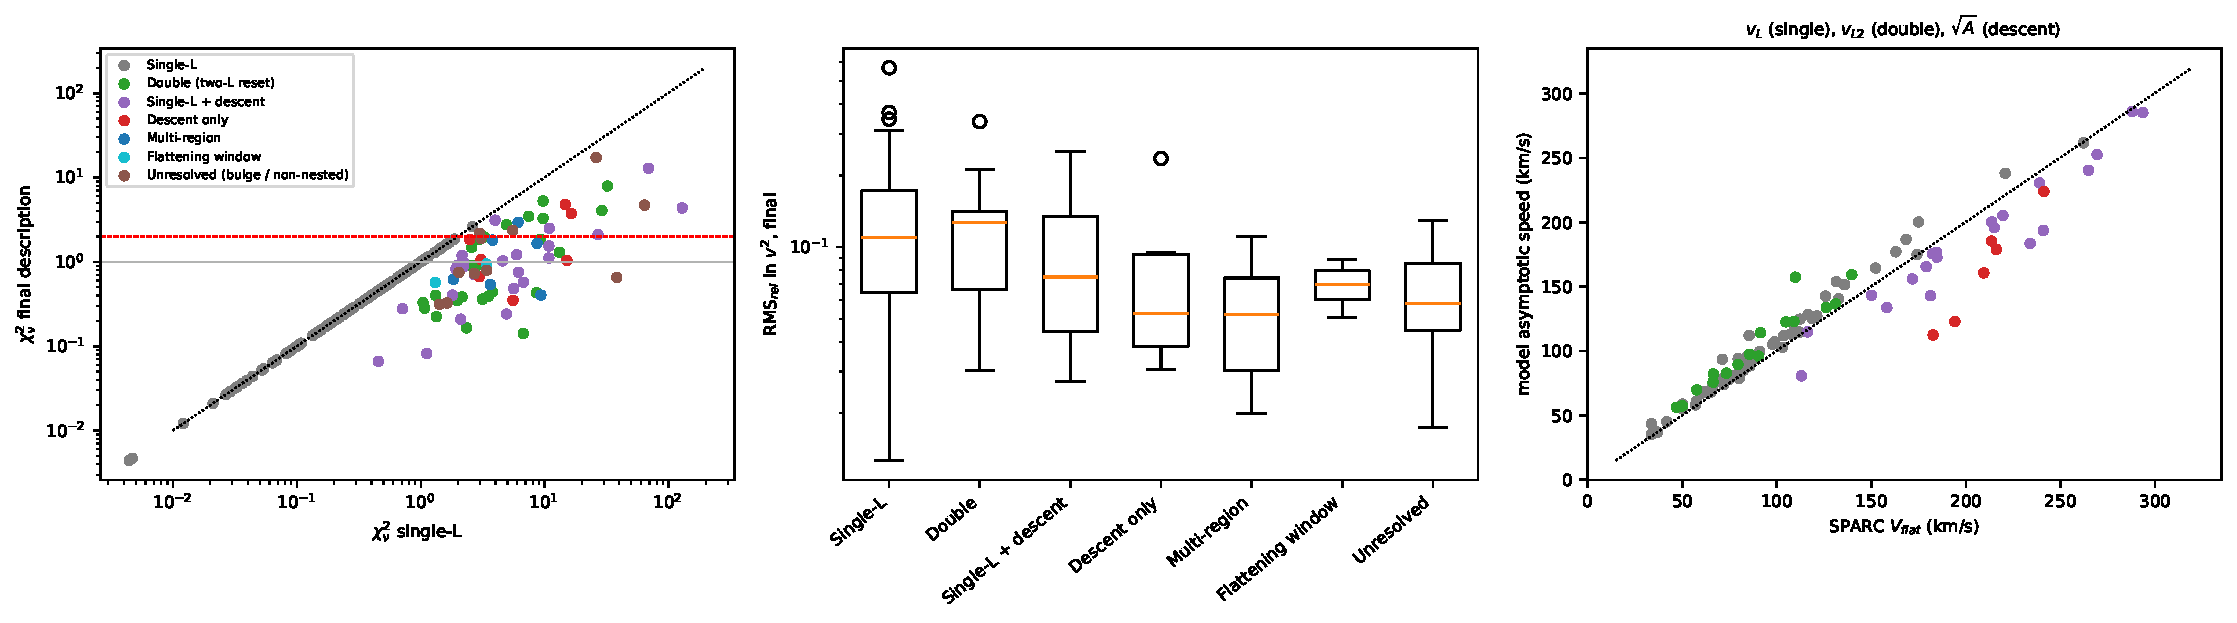
\includegraphics[width=\textwidth]{overall_fig_quality.pdf}\caption{Left: $\chi^2_\nu$ of single-L versus the final description. Middle: final RMS$_\mathrm{rel}$ per class. Right: model asymptotic speed ($v_L$ for single-L, $v_{L2}$ for nested two-L, $\sqrt A$ for descents) versus SPARC $V_\mathrm{flat}$.}\end{figure}
\begin{table}[h]\centering\small\caption{Fit quality per class (medians).}\begin{tabular}{lrrrrrrr}\toprule Class & $N$ & $n$ & $\chi^2_{\nu}$ single-L & $\chi^2_\nu$ final & RMS$_\mathrm{rel}$ final & final $\chi^2_\nu>2$ & $n\le13$\\\midrule
Single-L & 100 & 10 & 0.28 & 0.28 & 0.109 & 1 & 69\\
Double (two-L reset) & 25 & 21 & 3.26 & 0.90 & 0.127 & 6 & 8\\
Single-L + descent & 24 & 29 & 4.28 & 0.89 & 0.075 & 5 & 6\\
Descent only & 7 & 19 & 5.54 & 1.06 & 0.053 & 2 & 0\\
Multi-region & 6 & 23 & 4.94 & 1.14 & 0.052 & 1 & 1\\
Flattening window & 2 & 31 & 2.34 & 0.76 & 0.070 & 0 & 0\\
Unresolved (bulge / non-nested) & 11 & 28 & 3.06 & 0.80 & 0.058 & 4 & 2\\
All & 175 & 14 & 0.86 & 0.50 & 0.097 & 19 & 86\\\bottomrule\end{tabular}\end{table}
With the final descriptions, 156 of 175 galaxies have $\chi^2_\nu\le2$, and the median RMS$_\mathrm{rel}$ in $v^2$ is 0.097. The 19 galaxies above $\chi^2_\nu=2$ are DDO154, NGC1003, NGC2403, NGC3726, NGC4013, NGC5585, UGC03580, UGC06787, NGC2903, NGC5055, NGC5371, NGC5907, NGC6674, NGC6946, UGC02953, UGC11455, UGC00128, UGC09133, NGC4051. Apart from NGC 4051 ($n=7$, single-L with one deviant point), they are high-precision curves of two kinds: massive bulged spirals with a sharp inner peak (e.g.\ NGC 5055, UGC 2953, UGC 6787), and well-sampled nearby disks whose curves need more than one reset (NGC 2403, NGC 5585, NGC 1003, DDO 154). SPARC errors are conservative on average (median $\chi^2_\nu<1$ in all well-fitting classes), so $\chi^2_\nu$ is a weak discriminator within classes; RMS$_\mathrm{rel}$, residual structure and $\Delta\mathrm{BIC}$ are the more informative measures. The model asymptotic speed tracks $V_\mathrm{flat}$ in every class (right panel). The systematic offsets reflect whether the curve is still rising (single-L, double: model asymptote above $V_\mathrm{flat}$) or still descending (descent classes: floor below $V_\mathrm{flat}$) at the last measured point.
\section{Limitations}
\begin{enumerate}\itemsep1pt
\item \textbf{Thresholds.} Class boundaries depend on $\Delta\mathrm{BIC}<-6$ and on the physical screening rules. The seven undecided B galaxies and the borderline rising-window galaxies (NGC 300, NGC 6946) could move between Single-L and Double with more data.
\item \textbf{Short curves.} 86 galaxies have $n\le13$. For these the sign-based screen has little power, and a ``single-L'' classification often reflects data limitations.
\item \textbf{Heterogeneous selection.} The five analyses tested slightly different model sets: B tested two-L only, while C--E compared windows and two-L. A uniform re-run with all models on all galaxies would remove this dependence; by design it was not done here.
\item \textbf{Bulge description.} The unresolved class and most remaining residual structure point to the inner CL bulge. An explicit bulge component is the main open refinement.
\item \textbf{Model features.} The $v^2$ jump at a Lagrangian reset is not constrained by data. Window strengths $p$ are degenerate with $M$ when the descent dominates, so $M_N$ and $A$ should be quoted instead.
\item \textbf{Interpretation.} Associating windows with galaxy history, as proposed in [1], requires independent indicators (morphology, kinematic asymmetry, HI warps, environment); these were not part of the analyses.
\end{enumerate}
\section{Conclusions}
Starting from a two-parameter constant Lagrangian, 100 of 175 SPARC galaxies need nothing more. A further 56 are described by one additional, physically interpretable feature: a Lagrangian reset (late types) or a Keplerian descent (bulged spirals). 8 need two features or a flattening, and 11 bulge-dominated galaxies remain beyond the present model. The ordering of these classes along the Hubble sequence is the main empirical result. It ties the CL description to galaxy structure: the number and kind of Lagrangian regions follow the prominence of the bulge.

\section*{References}\small
[1] E.P.J.\ de Haas (2026), From Rotation Curves to Cosmic Time: Probing High-Redshift Expansion through Nested Spiral Dynamics, \emph{J.\ High Energy Phys.\ Grav.\ Cosmol.} 12, 334--367, doi:10.4236/jhepgc.2026.121022.\par
[2] E.P.J.\ de Haas, Galactic Rotation Curves and the Constant--Lagrangian Field: Empirical Tests within the $Q_g$ Rotor Framework (manuscript; single-L Eqs.~17--18, virial term Eq.~19, two-L Eqs.~24--26).\par
[3] F.\ Lelli, S.S.\ McGaugh, J.M.\ Schombert (2016), SPARC, \emph{AJ} 152, 157.\par
Category reports A--E (this project): CL\_categoryA\_report, CL\_categoryB\_report, CL\_categoryC\_report, CL\_categoryD\_report, CL\_categoryE\_report.

\clearpage\begin{landscape}{\scriptsize\setlength{\tabcolsep}{3pt}
\begin{longtable}{llllrrrrrrrl}
\caption{All 175 SPARC galaxies: overall class, origin, sub-type and fit quality (single-L $\to$ final). t = tentative ($n\le13$).}\\\toprule
Galaxy & Class & Sub-type & Cat. & Type & Q & $n$ & $\chi^2_{\nu}$ S & $\chi^2_\nu$ final & RMS final & $\Delta$BIC & Quality / grade\\\midrule\endfirsthead
\toprule Galaxy & Class & Sub-type & Cat. & Type & Q & $n$ & $\chi^2_{\nu}$ S & $\chi^2_\nu$ final & RMS final & $\Delta$BIC & Quality / grade\\\midrule\endhead\bottomrule\endfoot
CamB t & Single-L & adequate & A & Im & 2 & 9 & 0.04 & 0.04 & 0.044 & 0.0 & grade III\\
D512--2 t & Single-L & adequate & A & Im & 2 & 4 & 0.07 & 0.07 & 0.055 & 0.0 & grade II\\
D564--8 t & Single-L & adequate & A & Im & 2 & 6 & 0.15 & 0.15 & 0.092 & 0.0 & grade II\\
DDO170 t & Single-L & adequate & A & Im & 2 & 8 & 0.50 & 0.50 & 0.076 & 0.0 & grade II\\
F561--1 t & Single-L & adequate & A & Sm & 3 & 6 & 0.01 & 0.01 & 0.021 & 0.0 & grade II\\
F563--V1 t & Single-L & adequate & A & Im & 3 & 6 & 0.14 & 0.14 & 0.110 & 0.0 & grade III\\
F563--V2 t & Single-L & adequate & A & Im & 1 & 10 & 0.03 & 0.03 & 0.048 & 0.0 & grade I\\
F565--V2 t & Single-L & adequate & A & Im & 2 & 7 & 0.04 & 0.04 & 0.085 & 0.0 & grade II\\
F567--2 t & Single-L & adequate & A & Sm & 3 & 5 & 0.15 & 0.15 & 0.089 & 0.0 & grade II\\
F571--V1 t & Single-L & adequate & A & Sd & 2 & 7 & 0.04 & 0.04 & 0.060 & 0.0 & grade II\\
F574--2 t & Single-L & adequate & A & Sm & 3 & 5 & 0.03 & 0.03 & 0.143 & 0.0 & grade III\\
F583--1 & Single-L & adequate & A & Sm & 1 & 25 & 0.21 & 0.21 & 0.250 & 0.0 & grade I\\
F583--4 t & Single-L & adequate & A & Sc & 1 & 12 & 0.56 & 0.56 & 0.239 & 0.0 & grade I\\
NGC3877 t & Single-L & adequate & A & Sc & 2 & 13 & 0.15 & 0.15 & 0.062 & 0.0 & grade I\\
NGC3917 & Single-L & adequate & A & Scd & 1 & 17 & 0.40 & 0.40 & 0.040 & 0.0 & grade I\\
NGC3949 t & Single-L & adequate & A & Sbc & 2 & 7 & 0.03 & 0.03 & 0.019 & 0.0 & grade II\\
NGC3953 t & Single-L & adequate & A & Sbc & 1 & 8 & 0.52 & 0.52 & 0.048 & 0.0 & grade II\\
NGC4068 t & Single-L & adequate & A & Im & 2 & 6 & 0.08 & 0.08 & 0.077 & 0.0 & grade III\\
NGC4085 t & Single-L & adequate & A & Sc & 2 & 7 & 0.13 & 0.13 & 0.038 & 0.0 & grade II\\
NGC4389 t & Single-L & adequate & A & Sbc & 3 & 6 & 0.75 & 0.75 & 0.176 & 0.0 & grade II\\
NGC6789 t & Single-L & adequate & A & BCD & 2 & 4 & 0.58 & 0.58 & 0.258 & 0.0 & grade III\\
UGC02023 t & Single-L & adequate & A & Im & 2 & 5 & 0.08 & 0.08 & 0.172 & 0.0 & grade III\\
UGC02259 t & Single-L & adequate & A & Sdm & 2 & 8 & 0.66 & 0.66 & 0.052 & 0.0 & grade II\\
UGC04325 t & Single-L & adequate & A & Sm & 1 & 8 & 0.41 & 0.41 & 0.049 & 0.0 & grade II\\
UGC04483 t & Single-L & adequate & A & Im & 2 & 8 & 0.17 & 0.17 & 0.188 & 0.0 & grade I\\
UGC04499 t & Single-L & adequate & A & Sdm & 1 & 9 & 0.35 & 0.35 & 0.100 & 0.0 & grade I\\
UGC05005 t & Single-L & adequate & A & Im & 1 & 11 & 0.19 & 0.19 & 0.278 & 0.0 & grade I\\
UGC05414 t & Single-L & adequate & A & Im & 1 & 6 & 0.93 & 0.93 & 0.137 & 0.0 & grade II\\
UGC05750 t & Single-L & adequate & A & Sdm & 1 & 11 & 0.04 & 0.04 & 0.065 & 0.0 & grade I\\
UGC05918 t & Single-L & adequate & A & Im & 2 & 8 & 0.19 & 0.19 & 0.129 & 0.0 & grade II\\
UGC05999 t & Single-L & adequate & A & Im & 2 & 5 & 0.02 & 0.02 & 0.013 & 0.0 & grade II\\
UGC06399 t & Single-L & adequate & A & Sm & 1 & 9 & 0.22 & 0.22 & 0.111 & 0.0 & grade I\\
UGC06628 t & Single-L & adequate & A & Sm & 2 & 7 & 0.00 & 0.00 & 0.025 & 0.0 & grade II\\
UGC06667 t & Single-L & adequate & A & Scd & 1 & 9 & 0.72 & 0.72 & 0.145 & 0.0 & grade I\\
UGC06818 t & Single-L & adequate & A & Sm & 2 & 8 & 0.68 & 0.68 & 0.274 & 0.0 & grade I\\
UGC06917 t & Single-L & adequate & A & Sm & 1 & 11 & 0.74 & 0.74 & 0.086 & 0.0 & grade II\\
UGC06923 t & Single-L & adequate & A & Im & 2 & 6 & 0.71 & 0.71 & 0.226 & 0.0 & grade II\\
UGC06930 t & Single-L & adequate & A & Sd & 1 & 10 & 0.10 & 0.10 & 0.044 & 0.0 & grade II\\
UGC06973 t & Single-L & adequate & A & Sab & 3 & 9 & 0.36 & 0.36 & 0.036 & 0.0 & grade II\\
UGC07089 t & Single-L & adequate & A & Sdm & 2 & 12 & 0.70 & 0.70 & 0.199 & 0.0 & grade I\\
UGC07151 t & Single-L & adequate & A & Scd & 1 & 11 & 0.45 & 0.45 & 0.070 & 0.0 & grade I\\
UGC07232 t & Single-L & adequate & A & Im & 2 & 4 & 0.71 & 0.71 & 0.186 & 0.0 & grade III\\
UGC07261 t & Single-L & adequate & A & Sdm & 2 & 7 & 0.09 & 0.09 & 0.041 & 0.0 & grade II\\
UGC07559 t & Single-L & adequate & A & Im & 2 & 7 & 0.11 & 0.11 & 0.152 & 0.0 & grade II\\
UGC07577 t & Single-L & adequate & A & Im & 2 & 9 & 0.06 & 0.06 & 0.272 & 0.0 & grade III\\
UGC07603 t & Single-L & adequate & A & Sd & 1 & 12 & 0.46 & 0.46 & 0.126 & 0.0 & grade I\\
UGC07608 t & Single-L & adequate & A & Im & 1 & 8 & 0.16 & 0.16 & 0.092 & 0.0 & grade II\\
UGC07690 t & Single-L & adequate & A & Im & 2 & 7 & 0.66 & 0.66 & 0.103 & 0.0 & grade II\\
UGC07866 t & Single-L & adequate & A & Im & 2 & 7 & 0.21 & 0.21 & 0.170 & 0.0 & grade II\\
UGC08837 t & Single-L & adequate & A & Im & 2 & 8 & 0.05 & 0.05 & 0.041 & 0.0 & grade I\\
UGC09992 t & Single-L & adequate & A & Im & 2 & 5 & 0.00 & 0.00 & 0.018 & 0.0 & grade III\\
UGC10310 t & Single-L & adequate & A & Sm & 1 & 7 & 0.07 & 0.07 & 0.049 & 0.0 & grade II\\
UGC11557 t & Single-L & adequate & A & Sdm & 2 & 12 & 0.18 & 0.18 & 0.308 & 0.0 & grade I\\
UGCA281 t & Single-L & adequate & A & BCD & 3 & 7 & 0.29 & 0.29 & 0.186 & 0.0 & grade II\\
NGC3893 t & Single-L & extra scatter ($\sigma_\mathrm{int}$) & E & Sc & 1 & 10 & 1.45 & 1.45 & 0.128 & 0.0 & single-L kept\\
NGC4051 t & Single-L & extra scatter ($\sigma_\mathrm{int}$) & E & Sbc & 2 & 7 & 2.61 & 2.61 & 0.270 & 0.0 & single-L kept\\
UGC00634 t & Single-L & extra scatter ($\sigma_\mathrm{int}$) & E & Sm & 2 & 4 & 1.86 & 1.86 & 0.035 & 0.0 & single-L kept\\
UGC00891 t & Single-L & extra scatter ($\sigma_\mathrm{int}$) & E & Sm & 2 & 5 & 1.07 & 1.07 & 0.108 & 0.0 & single-L kept\\
UGC02455 t & Single-L & extra scatter ($\sigma_\mathrm{int}$) & E & Im & 3 & 8 & 1.60 & 1.60 & 0.369 & 0.0 & single-L kept\\
UGCA442 t & Single-L & extra scatter ($\sigma_\mathrm{int}$) & E & Sm & 1 & 8 & 1.47 & 1.47 & 0.214 & 0.0 & single-L kept\\
DDO064 & Single-L & structure within errors & D & Im & 1 & 14 & 0.24 & 0.24 & 0.306 & 0.0 & single-L adequate\\
F563--1 & Single-L & structure within errors & D & Sm & 1 & 17 & 0.24 & 0.24 & 0.166 & 0.0 & single-L adequate\\
NGC0024 & Single-L & structure within errors & D & Sc & 1 & 29 & 0.24 & 0.24 & 0.085 & 0.0 & single-L adequate\\
NGC2915 & Single-L & structure within errors & D & BCD & 2 & 30 & 0.26 & 0.26 & 0.123 & 0.0 & single-L adequate\\
PGC51017 t & Single-L & structure within errors & D & BCD & 3 & 6 & 0.21 & 0.21 & 0.096 & 0.0 & single-L adequate\\
UGC01281 & Single-L & structure within errors & D & Sdm & 1 & 25 & 0.03 & 0.03 & 0.065 & 0.0 & single-L adequate\\
NGC3109 & Single-L & undecided (-6$\le$dBIC$<$-2) & B & Sm & 1 & 25 & 0.78 & 0.78 & 0.127 & 0.0 & structured residuals\\
NGC3972 t & Single-L & undecided (-6$\le$dBIC$<$-2) & B & Sbc & 1 & 10 & 1.42 & 1.42 & 0.138 & 0.0 & structured residuals\\
NGC4010 t & Single-L & undecided (-6$\le$dBIC$<$-2) & B & Sd & 2 & 12 & 1.69 & 1.69 & 0.239 & 0.0 & structured residuals\\
UGC06446 & Single-L & undecided (-6$\le$dBIC$<$-2) & B & Sd & 1 & 17 & 0.67 & 0.67 & 0.147 & 0.0 & structured residuals\\
UGC07125 t & Single-L & undecided (-6$\le$dBIC$<$-2) & B & Sm & 1 & 13 & 1.15 & 1.15 & 0.150 & 0.0 & structured residuals\\
UGC07323 t & Single-L & undecided (-6$\le$dBIC$<$-2) & B & Sdm & 1 & 10 & 1.68 & 1.68 & 0.284 & 0.0 & structured residuals\\
UGC07399 t & Single-L & undecided (-6$\le$dBIC$<$-2) & B & Sdm & 1 & 10 & 1.29 & 1.29 & 0.098 & 0.0 & structured residuals\\
ESO079--G014 & Single-L & weak $+-+$ wave & B & Sbc & 1 & 15 & 1.12 & 1.12 & 0.345 & 0.0 & structured residuals\\
F568--1 t & Single-L & weak $+-+$ wave & B & Sc & 1 & 12 & 0.05 & 0.05 & 0.094 & 0.0 & structured residuals\\
F568--3 & Single-L & weak $+-+$ wave & B & Sd & 1 & 18 & 0.19 & 0.19 & 0.092 & 0.0 & structured residuals\\
F574--1 & Single-L & weak $+-+$ wave & B & Sd & 1 & 14 & 0.16 & 0.16 & 0.109 & 0.0 & structured residuals\\
F579--V1 & Single-L & weak $+-+$ wave & B & Sc & 1 & 14 & 0.10 & 0.10 & 0.108 & 0.0 & structured residuals\\
KK98--251 & Single-L & weak $+-+$ wave & B & Im & 2 & 15 & 0.18 & 0.18 & 0.066 & 0.0 & structured residuals\\
NGC0100 & Single-L & weak $+-+$ wave & B & Scd & 1 & 21 & 0.37 & 0.37 & 0.146 & 0.0 & structured residuals\\
NGC2976 & Single-L & weak $+-+$ wave & B & Sc & 2 & 27 & 0.47 & 0.47 & 0.155 & 0.0 & structured residuals\\
NGC4214 & Single-L & weak $+-+$ wave & B & Im & 2 & 14 & 0.53 & 0.53 & 0.122 & 0.0 & structured residuals\\
NGC5005 & Single-L & weak $+-+$ wave & B & Sbc & 1 & 18 & 0.20 & 0.20 & 0.087 & 0.0 & structured residuals\\
UGC05829 t & Single-L & weak $+-+$ wave & B & Im & 2 & 11 & 0.83 & 0.83 & 0.286 & 0.0 & structured residuals\\
UGC08286 & Single-L & weak $+-+$ wave & B & Scd & 1 & 17 & 0.15 & 0.15 & 0.028 & 0.0 & structured residuals\\
UGC08550 t & Single-L & weak $+-+$ wave & B & Sd & 1 & 11 & 0.68 & 0.68 & 0.061 & 0.0 & structured residuals\\
UGC12632 & Single-L & weak $+-+$ wave & B & Sm & 1 & 15 & 0.28 & 0.28 & 0.179 & 0.0 & structured residuals\\
UGCA444 & Single-L & weak $+-+$ wave & B & Im & 2 & 36 & 0.26 & 0.26 & 0.223 & 0.0 & structured residuals\\
F568--V1 & Single-L & weak $-+-$ wave & C & Sd & 1 & 15 & 0.08 & 0.08 & 0.145 & 0.0 & structured residuals\\
NGC1705 & Single-L & weak $-+-$ wave & C & BCD & 3 & 14 & 0.15 & 0.15 & 0.058 & 0.0 & structured residuals\\
NGC2366 & Single-L & weak $-+-$ wave & C & Im & 3 & 26 & 0.47 & 0.47 & 0.165 & 0.0 & structured residuals\\
NGC3769 t & Single-L & weak $-+-$ wave & C & Sb & 2 & 12 & 0.79 & 0.79 & 0.097 & 0.0 & structured residuals\\
NGC4183 & Single-L & weak $-+-$ wave & C & Scd & 1 & 23 & 0.54 & 0.54 & 0.145 & 0.0 & structured residuals\\
NGC4559 & Single-L & weak $-+-$ wave & C & Scd & 1 & 32 & 0.44 & 0.44 & 0.155 & 0.0 & structured residuals\\
UGC01230 t & Single-L & weak $-+-$ wave & C & Sm & 1 & 11 & 0.37 & 0.37 & 0.128 & 0.0 & structured residuals\\
UGC04305 & Single-L & weak $-+-$ wave & C & Im & 3 & 22 & 0.65 & 0.65 & 0.568 & 0.0 & structured residuals\\
UGC05721 & Single-L & weak $-+-$ wave & C & Sd & 1 & 23 & 1.01 & 1.01 & 0.222 & 0.0 & structured residuals\\
UGC06983 & Single-L & weak $-+-$ wave & C & Scd & 1 & 17 & 0.32 & 0.32 & 0.056 & 0.0 & structured residuals\\
UGC08490 & Single-L & weak $-+-$ wave & C & Sm & 1 & 30 & 0.50 & 0.50 & 0.103 & 0.0 & structured residuals\\
UGC09037 & Single-L & weak $-+-$ wave & C & Scd & 2 & 22 & 0.86 & 0.86 & 0.091 & 0.0 & structured residuals\\
\midrule
D631--7 & Double (two-L reset) & nested two-L & B & Im & 1 & 16 & 1.33 & 0.22 & 0.049 & -10.4 & grade I\\
DDO161 & Double (two-L reset) & nested two-L & B & Im & 1 & 31 & 2.15 & 0.38 & 0.096 & -45.1 & grade I\\
ESO116--G012 & Double (two-L reset) & nested two-L & B & Sd & 1 & 15 & 2.57 & 1.49 & 0.194 & -11.7 & grade II\\
F571--8 t & Double (two-L reset) & nested two-L & B & Sc & 1 & 13 & 3.79 & 0.44 & 0.132 & -32.6 & grade II\\
IC2574 & Double (two-L reset) & nested two-L & B & Sm & 2 & 34 & 13.13 & 1.30 & 0.107 & -374.1 & grade I\\
NGC0055 & Double (two-L reset) & nested two-L & B & Sm & 2 & 21 & 1.04 & 0.33 & 0.056 & -8.1 & grade II\\
NGC0247 & Double (two-L reset) & nested two-L & B & Sd & 2 & 26 & 8.58 & 0.43 & 0.038 & -189.9 & grade II\\
NGC3741 & Double (two-L reset) & nested two-L & B & Im & 1 & 21 & 3.52 & 0.39 & 0.134 & -54.0 & grade I\\
NGC7793 & Double (two-L reset) & nested two-L & B & Sd & 1 & 46 & 2.57 & 0.90 & 0.213 & -67.5 & grade I\\
UGC00731 t & Double (two-L reset) & nested two-L & B & Im & 1 & 12 & 2.34 & 0.16 & 0.030 & -17.1 & grade II\\
UGC04278 & Double (two-L reset) & nested two-L & B & Sd & 1 & 25 & 1.97 & 0.35 & 0.141 & -31.6 & grade I\\
UGC07524 & Double (two-L reset) & nested two-L & B & Sm & 1 & 31 & 1.07 & 0.28 & 0.127 & -16.6 & grade II\\
UGC12732 & Double (two-L reset) & nested two-L & B & Sm & 1 & 16 & 2.81 & 0.90 & 0.127 & -23.0 & grade II\\
DDO168 t & Double (two-L reset) & rising window (p$<$0) & E & Im & 2 & 10 & 2.92 & 1.84 & 0.142 & -7.7 & weakly constrained\\
ESO444--G084 t & Double (two-L reset) & rising window (p$<$0) & E & Im & 2 & 7 & 3.14 & 0.36 & 0.066 & -10.7 & weakly constrained\\
NGC0300 & Double (two-L reset) & rising window (p$<$0) & D & Sd & 2 & 25 & 1.31 & 0.40 & 0.065 & -15.4 & clean\\
NGC6946 & Double (two-L reset) & rising window (p$<$0) & C & Scd & 1 & 58 & 9.71 & 5.27 & 0.173 & -251.4 & rising window\\
UGC00191 t & Double (two-L reset) & rising window (p$<$0) & E & Sm & 1 & 9 & 3.26 & 1.97 & 0.109 & -8.5 & weakly constrained\\
UGC05716 t & Double (two-L reset) & rising window (p$<$0) & E & Sm & 2 & 12 & 9.28 & 1.85 & 0.049 & -73.0 & clean\\
UGC11820 t & Double (two-L reset) & rising window (p$<$0) & E & Sm & 1 & 10 & 6.72 & 0.14 & 0.159 & -48.3 & clean\\
DDO154 t & Double (two-L reset) & two-L, needs more regions & B & Im & 2 & 12 & 7.43 & 3.48 & 0.141 & -41.6 & grade IIM\\
NGC1003 & Double (two-L reset) & two-L, needs more regions & B & Scd & 1 & 36 & 4.91 & 2.77 & 0.114 & -71.2 & grade IM\\
NGC2403 & Double (two-L reset) & two-L, needs more regions & B & Scd & 1 & 73 & 32.04 & 7.93 & 0.105 & -1719.3 & grade IM\\
NGC5585 & Double (two-L reset) & two-L, needs more regions & B & Sd & 1 & 24 & 28.93 & 4.05 & 0.127 & -549.1 & grade IIM\\
UGC03580 & Double (two-L reset) & two-L, needs more regions & B & Sa & 2 & 47 & 9.69 & 3.29 & 0.337 & -286.9 & grade IM\\
\midrule
NGC0801 t & Single-L + descent & CL + Kepler descent & E & Sc & 1 & 13 & 10.80 & 1.54 & 0.074 & -99.8 & clean\\
NGC2683 t & Single-L + descent & CL + Kepler descent & E & Sb & 2 & 11 & 10.79 & 1.11 & 0.088 & -84.6 & weakly constrained\\
NGC2903 & Single-L + descent & CL + Kepler descent & C & Sbc & 1 & 34 & 26.86 & 2.10 & 0.100 & -789.5 & grade IM\\
NGC2998 t & Single-L + descent & CL + Kepler descent & E & Sc & 1 & 13 & 1.98 & 0.91 & 0.253 & -8.5 & weakly constrained\\
NGC3198 & Single-L + descent & CL + Kepler descent & C & Sc & 1 & 43 & 6.13 & 0.75 & 0.224 & -214.2 & grade I\\
NGC3521 & Single-L + descent & CL + Kepler descent & C & Sbc & 1 & 41 & 0.45 & 0.07 & 0.039 & -7.8 & grade III\\
NGC3992 t & Single-L + descent & CL + Kepler descent & C & Sbc & 1 & 9 & 5.62 & 0.48 & 0.029 & -32.5 & grade I\\
NGC4088 t & Single-L + descent & CL + Kepler descent & C & Sbc & 1 & 12 & 1.81 & 0.40 & 0.076 & -9.9 & grade III\\
NGC4100 & Single-L + descent & CL + Kepler descent & C & Sbc & 1 & 24 & 6.72 & 0.57 & 0.050 & -130.0 & grade I\\
NGC4138 t & Single-L + descent & CL + Kepler descent & D & S0 & 2 & 7 & 4.91 & 0.24 & 0.072 & -19.9 & weakly constrained\\
NGC4157 & Single-L + descent & CL + Kepler descent & C & Sb & 1 & 17 & 2.10 & 0.21 & 0.052 & -23.1 & grade II\\
NGC4217 & Single-L + descent & CL + Kepler descent & C & Sb & 1 & 19 & 1.11 & 0.08 & 0.036 & -11.8 & grade III\\
NGC5055 & Single-L + descent & CL + Kepler descent & C & Sbc & 1 & 28 & 128.68 & 4.36 & 0.120 & -3234.6 & grade IM\\
NGC5907 & Single-L + descent & CL + Kepler descent & C & Sc & 1 & 19 & 10.88 & 2.50 & 0.036 & -141.6 & grade IIM\\
NGC5985 & Single-L + descent & CL + Kepler descent & C & Sb & 1 & 33 & 2.20 & 0.88 & 0.038 & -35.9 & grade III\\
NGC6503 & Single-L + descent & CL + Kepler descent & C & Scd & 1 & 31 & 1.92 & 0.82 & 0.046 & -26.5 & grade II\\
NGC7331 & Single-L + descent & CL + Kepler descent & C & Sb & 1 & 36 & 2.70 & 0.71 & 0.027 & -62.2 & grade II\\
UGC02953 & Single-L + descent & CL + Kepler descent & C & Sab & 2 & 115 & 68.64 & 12.87 & 0.248 & -6317.8 & grade IM\\
UGC03205 & Single-L + descent & CL + Kepler descent & C & Sab & 1 & 48 & 5.93 & 1.21 & 0.169 & -211.8 & grade II\\
UGC05986 & Single-L + descent & CL + Kepler descent & C & Sm & 2 & 15 & 2.15 & 1.20 & 0.126 & -9.4 & grade III\\
UGC08699 & Single-L + descent & CL + Kepler descent & C & Sab & 2 & 41 & 4.58 & 1.03 & 0.070 & -133.3 & grade II\\
UGC11455 & Single-L + descent & CL + Kepler descent & C & Scd & 1 & 36 & 3.97 & 3.12 & 0.170 & -28.0 & grade IIIM\\
UGC11914 & Single-L + descent & CL + Kepler descent & C & Sab & 1 & 65 & 2.22 & 0.99 & 0.097 & -70.9 & grade III\\
UGC12506 & Single-L + descent & CL + Kepler descent & C & Scd & 2 & 31 & 0.71 & 0.28 & 0.163 & -6.2 & grade III\\
\midrule
NGC7814 & Descent only & descent from first points & D & Sab & 1 & 18 & 2.96 & 0.67 & 0.031 & -32.3 & weakly constrained\\
NGC0891 & Descent only & descent-dominated & C & Sb & 1 & 18 & 3.06 & 1.06 & 0.091 & -28.2 & grade III\\
NGC5033 & Descent only & descent-dominated & C & Sc & 1 & 22 & 15.11 & 1.04 & 0.042 & -277.3 & grade III\\
NGC5371 & Descent only & descent-dominated & C & Sbc & 1 & 19 & 14.64 & 4.79 & 0.095 & -171.2 & grade IIIM\\
NGC6674 & Descent only & descent-dominated & C & Sb & 1 & 15 & 16.38 & 3.74 & 0.236 & -166.4 & grade IIM\\
UGC02916 & Descent only & descent-dominated & C & Sab & 2 & 43 & 2.48 & 1.84 & 0.053 & -22.5 & grade III\\
UGC05253 & Descent only & descent-dominated & C & Sab & 2 & 73 & 5.54 & 0.35 & 0.034 & -360.7 & grade I\\
\midrule
NGC1090 & Multi-region & reset + disk window & D & Sbc & 1 & 24 & 3.63 & 0.54 & 0.077 & -57.5 & weakly constrained\\
NGC6015 & Multi-region & reset + disk window & D & Scd & 2 & 44 & 8.66 & 1.66 & 0.064 & -285.8 & clean\\
NGC2841 & Multi-region & two windows & D & Sb & 1 & 50 & 9.31 & 0.40 & 0.020 & -413.3 & clean\\
NGC6195 & Multi-region & two windows & E & Sb & 1 & 23 & 1.83 & 0.62 & 0.039 & -15.4 & weakly constrained\\
UGC00128 & Multi-region & two windows & D & Sdm & 1 & 22 & 6.09 & 2.95 & 0.111 & -62.4 & weakly constrained\\
UGC05764 t & Multi-region & two windows & E & Im & 2 & 10 & 3.79 & 1.81 & 0.027 & -13.9 & weakly constrained\\
\midrule
ESO563--G021 & Flattening window & 0$<$p$<$2 & C & Sbc & 1 & 30 & 3.38 & 0.94 & 0.089 & -63.3 & --\\
IC4202 & Flattening window & 0$<$p$<$2 & C & Sbc & 1 & 32 & 1.31 & 0.57 & 0.051 & -16.3 & --\\
\midrule
NGC0289 & Unresolved (bulge / non-nested) & extreme window parameters & D & Sbc & 2 & 28 & 2.70 & 0.73 & 0.080 & -40.9 & phenomenological\\
NGC2955 & Unresolved (bulge / non-nested) & extreme window parameters & E & Sb & 1 & 24 & 3.06 & 1.91 & 0.065 & -20.2 & phenomenological\\
UGC02487 & Unresolved (bulge / non-nested) & extreme window parameters & D & S0 & 1 & 17 & 38.15 & 0.66 & 0.026 & -553.7 & phenomenological\\
UGC03546 & Unresolved (bulge / non-nested) & extreme window parameters & D & Sa & 1 & 30 & 3.40 & 0.80 & 0.058 & -62.6 & phenomenological\\
UGC06786 & Unresolved (bulge / non-nested) & extreme window parameters & D & S0 & 1 & 45 & 1.41 & 0.31 & 0.018 & -33.2 & phenomenological\\
UGC09133 & Unresolved (bulge / non-nested) & extreme window parameters & D & Sab & 1 & 68 & 64.01 & 4.71 & 0.035 & -3915.8 & phenomenological\\
NGC3726 t & Unresolved (bulge / non-nested) & two-L non-nested & B & Sc & 2 & 12 & 2.98 & 2.19 & 0.091 & -7.3 & flag N\\
NGC4013 & Unresolved (bulge / non-nested) & two-L non-nested & B & Sb & 2 & 36 & 5.52 & 2.36 & 0.118 & -104.9 & flag N\\
UGC02885 & Unresolved (bulge / non-nested) & two-L non-nested & B & Sc & 1 & 19 & 2.03 & 0.75 & 0.056 & -17.3 & flag N\\
UGC06614 t & Unresolved (bulge / non-nested) & two-L non-nested & B & Sa & 1 & 13 & 1.62 & 0.33 & 0.054 & -9.8 & flag N\\
UGC06787 & Unresolved (bulge / non-nested) & two-L non-nested & B & Sab & 2 & 71 & 25.98 & 17.26 & 0.129 & -627.4 & flag N\\
\end{longtable}}\end{landscape}\end{document}